% created on 30/03/2020
% @author : ebazan
\part{Color of the Textures}\label{part:local_color_of_texture}

\section*{Introduction}
We dedicate part \ref{part:global_color_texture} of this thesis to the study of the global distribution of color and texture information. In the case of color, we emphasize the importance of choosing a perceptual color space, while for texture, we show that Gabor filters satisfactorily characterize the properties of homogeneous textures. We show the aforementioned through two image retrieval systems that use color and texture information in conjunction with EMD to retrieve the most similar images. We also show that EMD is a metric that reflects the similarity between distributions in a perceptual way.

However, the understanding of scenes (in a general way but particulary in the context of UAVs), is a more complex problem compared to the image retrieval systems presented in the previous part.
First, the distribution of color and texture information in natural images is more complex. Since we are dealing with non-homogeneous images, it is very possible that an image has objects with different colors and / or textures. In addition, it is possible that one feature generates or is implicit in the other. For example, a repetitive variation between two colors seen very closely can be perceived as two objects, while seen at a longer distance, it can be perceived as the texture of a more complex object.

In this final part of the thesis, we use the color and texture information again but in a different way. We explore the spectral decomposition of an image in a complex color space. With this strategy we recover the local texture information of the objects in an image taking into account the luminance and chrominance information of the scene.

This technique generates a space of balanced fetaures that allows to recover the perceptual contours of the objects in an image and consequently their segmentation. We show the versatility of this space using different techniques for object segmentation. While this framework is totally unsupervised, we show that it is also useful in identifying the importance of color and texture in human-made segmentations. Finally, we show that it is possible to obtain high-level features from this spectral decomposition.

The main contributions of this part are:
\begin{enumerate}
	\item Extensive analysis of gabor filters and their properties in the space-frequency domains.
	\item Interactive tool for custom generation of 2D Gabor filters.
	\item Generation of a feature space that includes the color and texture information of an image.
	\item Unsupervised framework for natural image segmentation.
	\item Tool for the interactive segmentation of images considering the information of color and texture.
\end{enumerate}

\chapter{Spectral Decomposition of an Image}\label{ch:spectral_image_decomposition}

\section*{Résumé}
\noindent Dans ce chapitre, nous utilisons la théorie du signal et l'analyse de Fourier pour générer une famille optimisée de filtres de Gabor. Le but est de récupérer autant d'informations que possible sur les textures d'une image dans le domaine fréquentiel sans affecter la localisation des informations. Nous présentons une analyse de la fonction de Gabor conforme au principe d'incertitude de Heisenberg. La méthodologie présentée dans ce chapitre générera des banques de filtres Gabor entièrement personnalisées. 

\section*{Abstract}
\noindent In this chapter we use signal theory and Fourier analysis to generate an optimized family of Gabor filters. The goal is to retrieve as much information as possible about textures from an image in the frequency domain without affecting the location of the information. We present an analysis of the Gabor function that complies with the Heisenberg uncertainty principle. The methodology presented in this chapter will generate fully customized Gabor filter banks. 

\section{Introduction}

The study and understanding of human vision has contributed to computer vision. Through neuropsychology, mathematical interpretations of the visual system have been developed, in particular of the first area of the primary visual cortex, the so-called V1.

Novel experimental techniques \citep{DeAngelis.Ohzawa.ea:TN:1995} have made it possible to observe the activity of V1 and of the modules involved in visual processes. It is known that the Receptive Field (RF) is in charge of formatting the optical signals for their interpretation. Physically, RF is the area of a visual neuron which responds to specific light stimuli. The RF response is known as the Receptive Profile (PR) and it can be positive and exciting or negative and exciting. The figure \ref{fig:V1_RP} shows the level curves of the receptor profile of a neuron, showing positive responses in green and negative responses in red.
Mathematically the RP is a function $\varphi:  D \rightarrow \mathbb{R}$ that is defined in the domain $D$ of the RF and measures the response $\varphi(x,y)$ of the neuron (positive or negative) to the stimulations at the point $(x,y)$ \citep{Petitot:Neurogeometrie:2008}.
The transfer function of a neuron $\varphi(x,y)$ can be considered as a filter, e.g. the Gabor filter, that correctly replicates the behavior of the V1 receptive profil (see Fig. \ref{fig:V1_RP_Gabor}).

\begin{figure}[!ht] 
	\centering
	\begin{subfigure}[b]{0.4\textwidth}
		\centering
		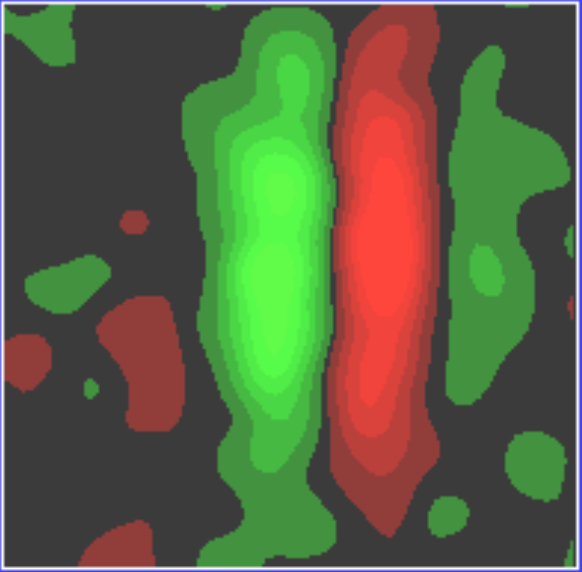
\includegraphics[width=\textwidth]{V1_RP2}
		\caption{Experimental level curves of RP}	
		\label{fig:V1_RP}
	\end{subfigure}
	\qquad %add desired spacing between images, e. g. ~, \quad, \qquad, \hfill etc. 
	%(or a blank line to force the subfigure onto a new line)
	\begin{subfigure}[b]{0.4\textwidth}
		\centering
		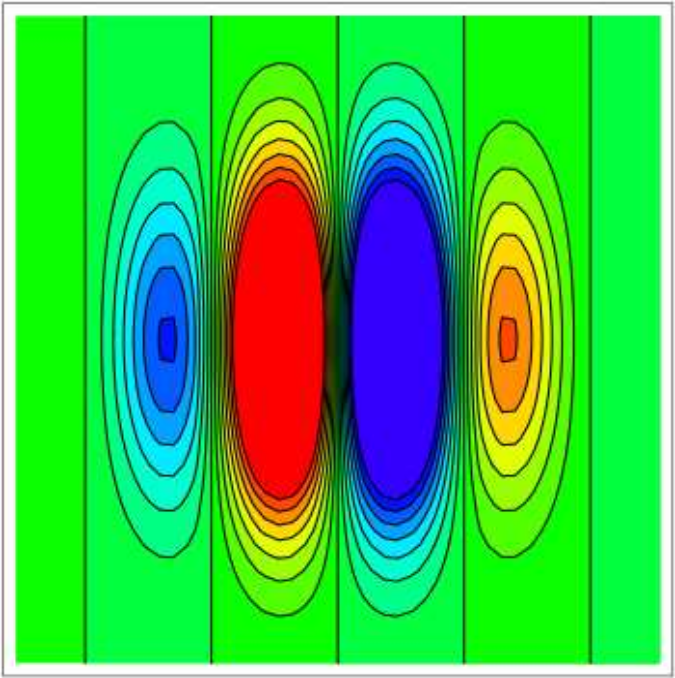
\includegraphics[width=\textwidth]{V1_RP_Gabor_model2}
		\caption{Gabor model of a RP }	
		\label{fig:V1_RP_Gabor}
	\end{subfigure}

  \caption{Receptive Profil of a simple visual neuron. Images from \citep{Petitot:Neurogeometrie:2008}}
  \label{fig:simple_neuron_receptive_profil}
\end{figure}

In Chapter \ref{ch:similarity_measures} we use the Gabor filter to extract global energy from homogeneous, i.e., stationary textures. This energy serves as the characteristic signature of the texture present in the image. In this chapter, motivated by its relationship with the human perception process, we delve into the study of Gabor filters. In particular, we are interested in its space-frequency properties for the extraction of local texture features in natural images.

We carry out an analysis of the Gabor filters first from the point of view of signal theory to expose their properties and limits. Then, starting from the representation of the filters in 1-d, we propose a formulation of the filters that allows us to fully customize a family of 2-d filters depending on the application. Especially the reformulation of Gabor filters allows to deal with aliasing and DC component problems (is this a conclusion?).

Using a family of Gabor filters, we generate a feature bank that contains local information about the texture. As natural images generally contain color information, the proposed framework allows obtaining local texture features taking into account the luminance and chrominance (if any) of an image.

\section{The Gabor filter as a measurement tool}\label{ch:gabor_filter_description}

In this section we present a reminder of the signal theory applied to image processing for feature extraction and object detection. First, we show what are the reasons for restricting signal analysis in two predefined domains: time and frequency (for the 1-d case) and space and frequency (for the 2-d case). We especially recall Gabor's filter theory and properties by showing how these filters are related to Heisneberg's uncertainty principle.

As we mentioned before, we use Gabor filters as a tool to measure the information that characterizes a signal. Since the signal information can relevant information at different points and scales (either in the spatial or space-frequency domain), a well-known strategy used in the literature is to create a filter bank that covers most of the spectrum to be able to reconstruct the original signal.

\subsection{Signals in two domains}
In the field of signal and image processing there are two popular ways to describe signals (one-dimensional (1-d) or two-dimensional (2-d)). The first consists of representing the signal as a function of time, while the second represents it as a function of frequency. These two representations carry the same signal information but in different ways, moreover, we can go from one to another via the Fourier transform (or the inverse Fourier transform), which makes these descriptions of special interest.We define the pair of 1-d Fourier transforms (FT) as follows
\begin{equation}\label{eq:fourier_transforms_1d}
    \begin{gathered}
        H(\upsilon) = \mathcal{F}\{h(t)\} = \int_{-\infty}^{\infty} h(t) e^{-j2\pi f t} dt \\
        h(t) = \mathcal{F}^{-1}\{H(\upsilon)\} = \int_{-\infty}^{\infty} H(\upsilon) e^{j2\pi f t} df 
    \end{gathered}
\end{equation}
while for the 2-d case, we define the FT as

\begin{equation}\label{eq:fourier_transforms_2d}
    \begin{gathered}
        H(u, v) = \mathcal{F}\{h(x, y)\} = \int_{-\infty}^{\infty} \int_{-\infty}^{\infty} h(x, y) e^{-j2\pi (ux + vy)} dx dy \\
        h(x, y) = \mathcal{F}^{-1}\{H(u, v)\} = \int_{-\infty}^{\infty} \int_{-\infty}^{\infty}  H(u, v) e^{j2\pi (ux + vy)} du dv 
    \end{gathered}
\end{equation}

Both representations of the signal are somewhat ideal, since the first operates at defined instants of time while the second operates on an infinite series of successive waves at defined frequencies \citep{Gabor:JIEE:1946}. 

It is evident that the function $h(t)$ (resp. $h(x, y)$) is located in both domains, however, it is also well known that no signal with compact support cannot have a finite Fourier transform and vice versa \citep{Bracewell:FourierBook:1999}, there is a certain uncertainty in the time and frequency locations of $h(t)$ (resp. space and frequency locations of $h(x, y)$). We developed and demonstrated the principle that defines this uncertainty (for signal processing and image processing) in appendix \ref{ch:uncertainty_principle} of this document.

\subsection{1-d Gabor filters}
The uncertainty principle shows that time and frequency are two fundamental domains and physically measurable quantities, but still idealizations if one is considered from the other's perspective.
Frequency is a simple waveform in the time domain, but to be sharply defined in the frequency domain it must be infinite in the time domain; a waveform always existed and remains forever. In everyday life it is very difficult to find phenomena with these characteristics, it is more common to find signals that have properties from both domains; certainly they have some frequency characteristics, but they also have a starting point and after some time these signals begin to fade away. This was the motivation of Dennis Gabor to represent signals simultaneously in time and frequency through the Gabor Elementary Function (GEF) \citep{Gabor:JIEE:1946}. The function represents the minimal quantum of information, i.e., the minimal amount of simultaneous information in time and frequency. In other words, it occupies the minimal area, given by a rectangle, in the time-frequency plane.  

The Gabor function is derived form the uncertainty principle (see \ref{ch:uncertainty_principle}), therefore, it has a shape for which the product $\Delta t \Delta \upsilon$ assumes the smallest possible value. In other words, the Gabor function is the one that transforms inequality of Eq. \eqref{eq:uncertainty_principle_freq} into the equality $\Delta t \Delta \upsilon = \frac{1}{4 \pi}$. This function is then defined as the modulation product of a harmonic oscillation (a sinusoidal wave) of any frequency with pulse of the form of a probability function (a Gaussian function) \citep{Gabor:JIEE:1946} and it and is represented as
\begin{equation}\label{eq:gabor_function_1d_time}
    g(t) =  e ^{-\alpha^2(t-t_0)^2} e ^{j 2 \pi f t + \phi}
\end{equation}
where $\alpha$ express the \textit{spread} and $t_0$ denotes the centroid of the Gaussian function, $f$ is the frequency of the sinusoidal wave, and $\phi$ defines the phase shift of the oscillation.

The representation of the Gabor function in the frequency domain is defined by the Fourier transform of \eqref{eq:gabor_function_1d_time} $G(\upsilon) = \mathcal{F}\{g(t)\}$ with the following analytical form

\begin{equation}\label{eq:gabor_function_1d_freq}
    G(\upsilon) =  \sqrt{\frac{\pi}{\alpha^2}} e ^{-\left(\frac{\pi}{\alpha}\right) ^{2} (\upsilon-f)^2} e ^{-j 2 \pi t_0 (\upsilon-f) + \phi}
\end{equation}

The equations \eqref{eq:gabor_function_1d_time} and \eqref{eq:gabor_function_1d_freq} show straightforward that the center of gravity $t_0$ is equal to \eqref{eq:center_of_gravity} and the spectral center of gravity $f$ is equal to \eqref{eq:spectral_center_of_gravity}, i.e., the Gabor functions follow the Heisenberg's uncertainty principle.   

\begin{figure}[!ht] 
	\centering
	\begin{subfigure}[b]{0.23\textwidth}
		\centering
		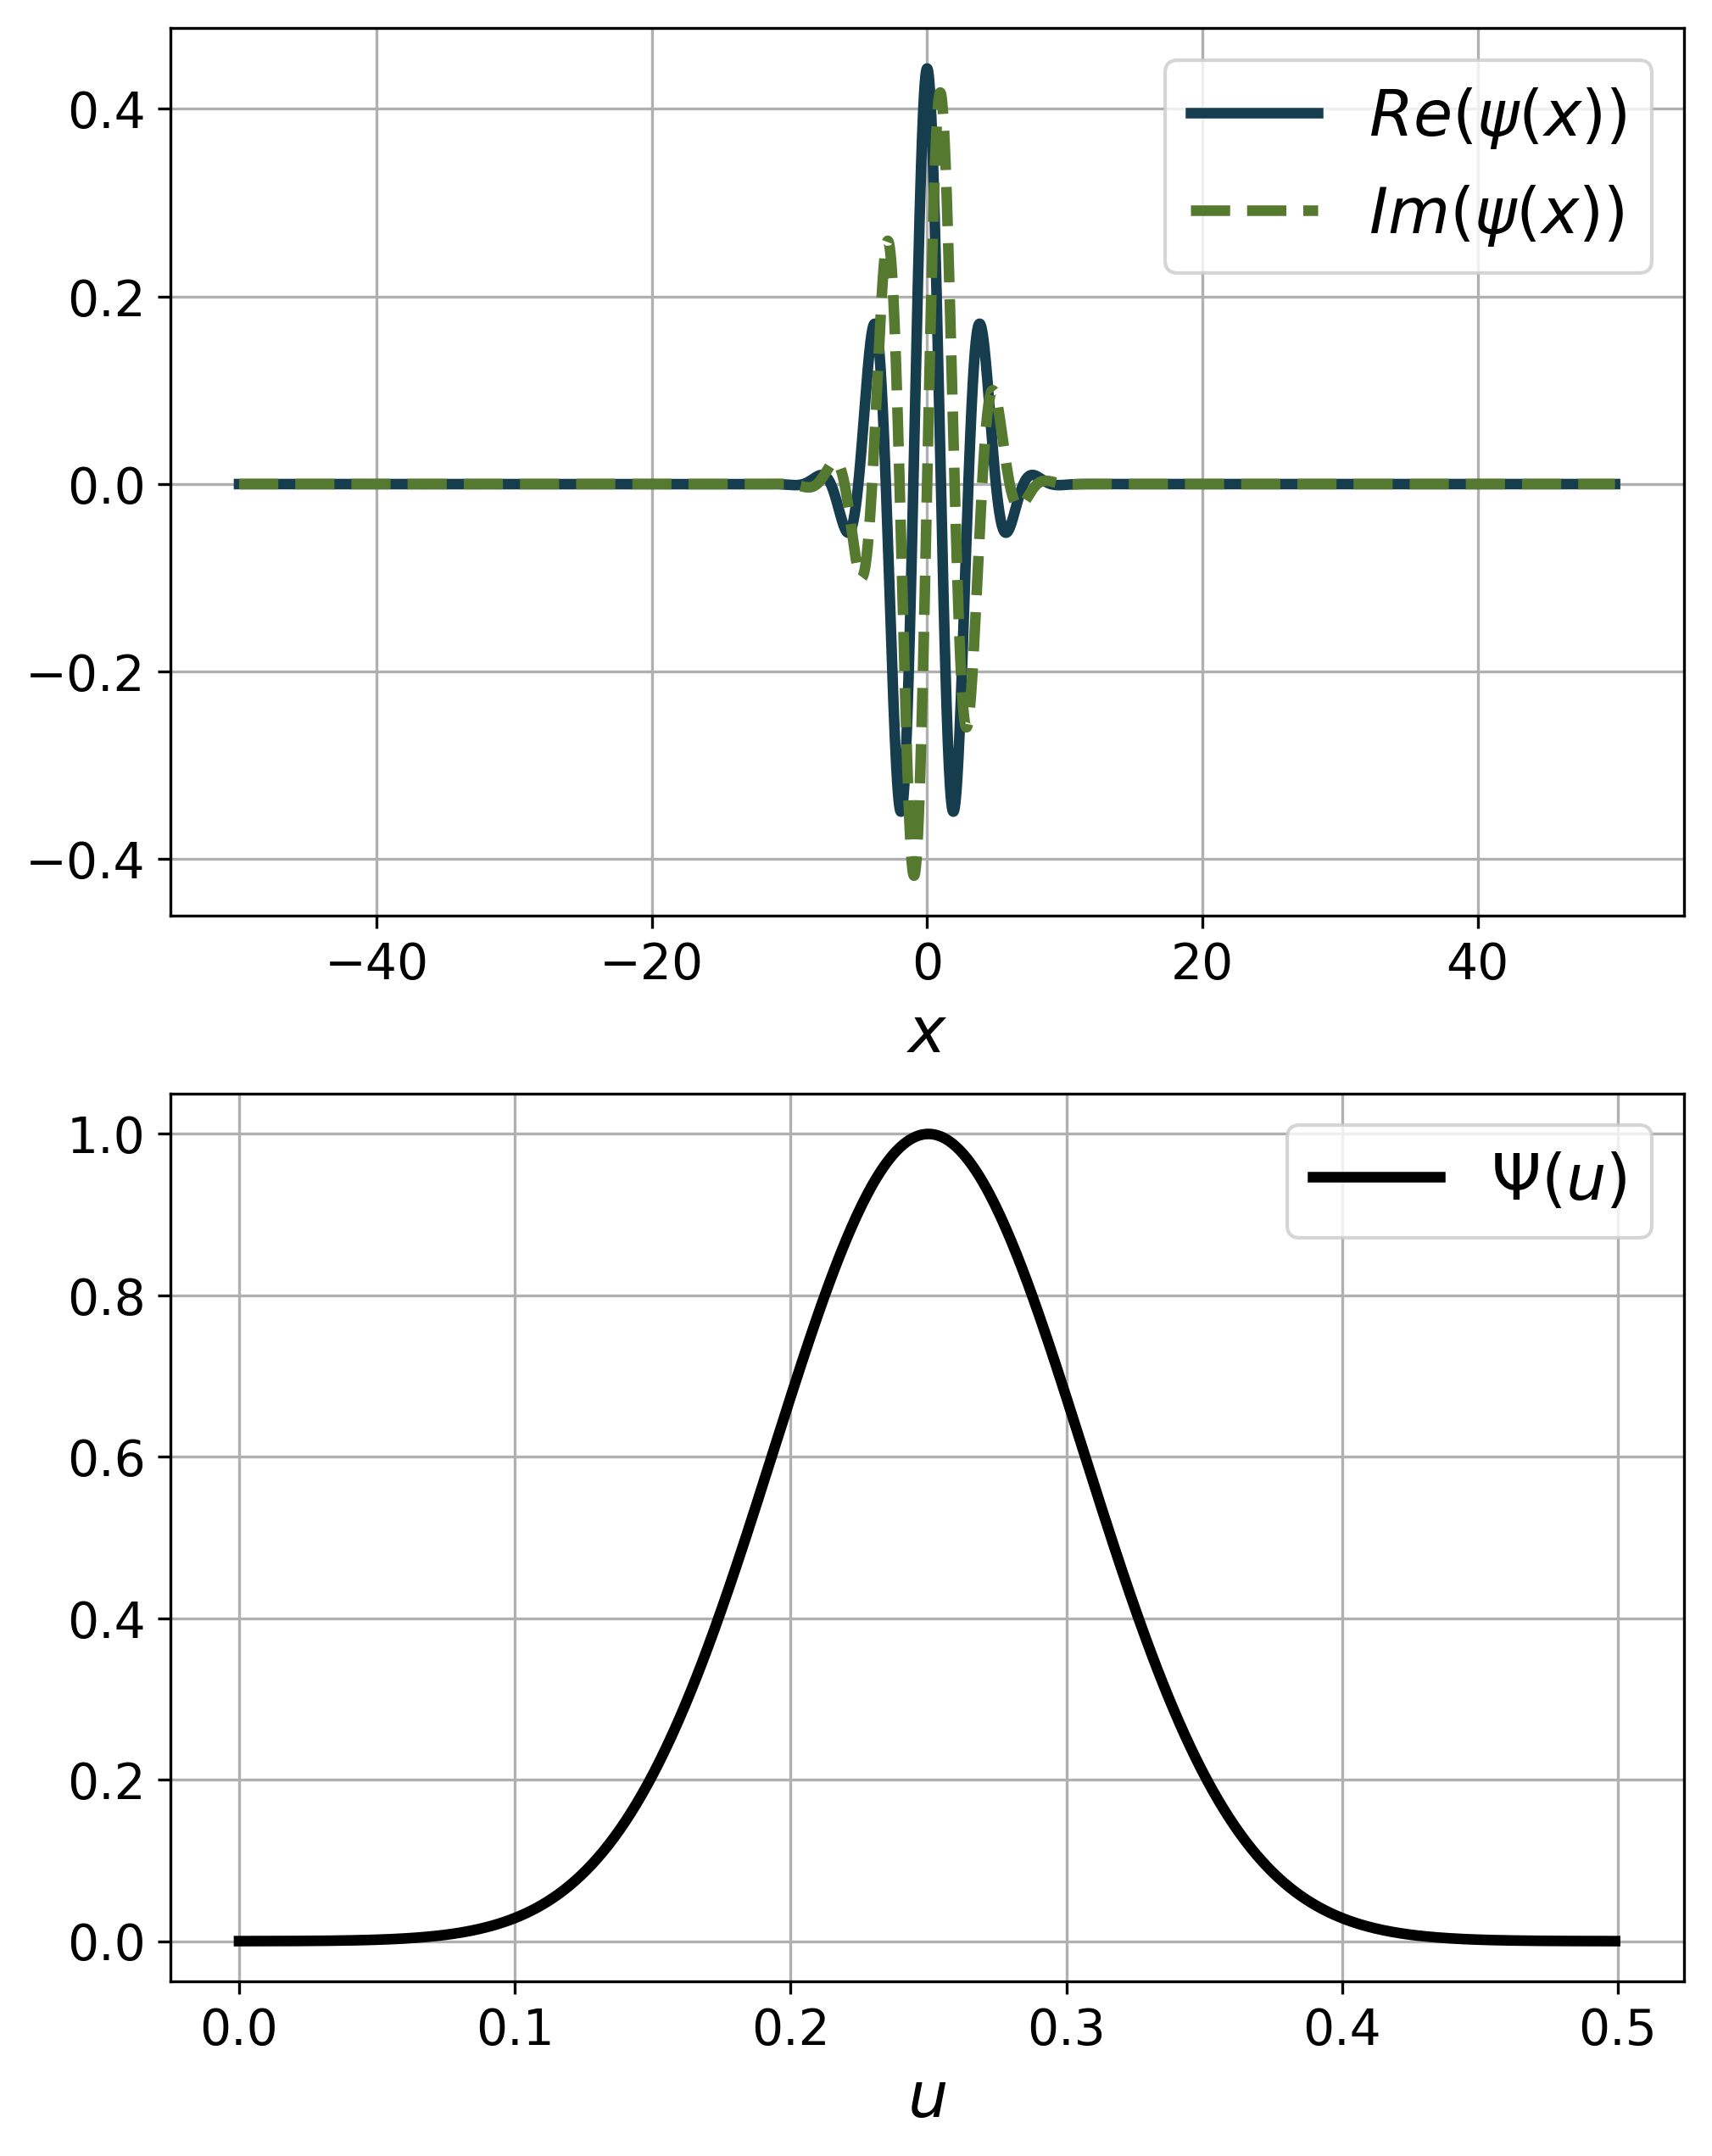
\includegraphics[width=\textwidth]{1D_GaborFilter_ver_f4_g1}
		\caption{}
		\label{fig:1D_GaborFilter_f4_g1}
	\end{subfigure}
	%add desired spacing between images, e. g. ~, \quad, \qquad, \hfill etc. 
	%(or a blank line to force the subfigure onto a new line)
	\begin{subfigure}[b]{0.23\textwidth}
		\centering
		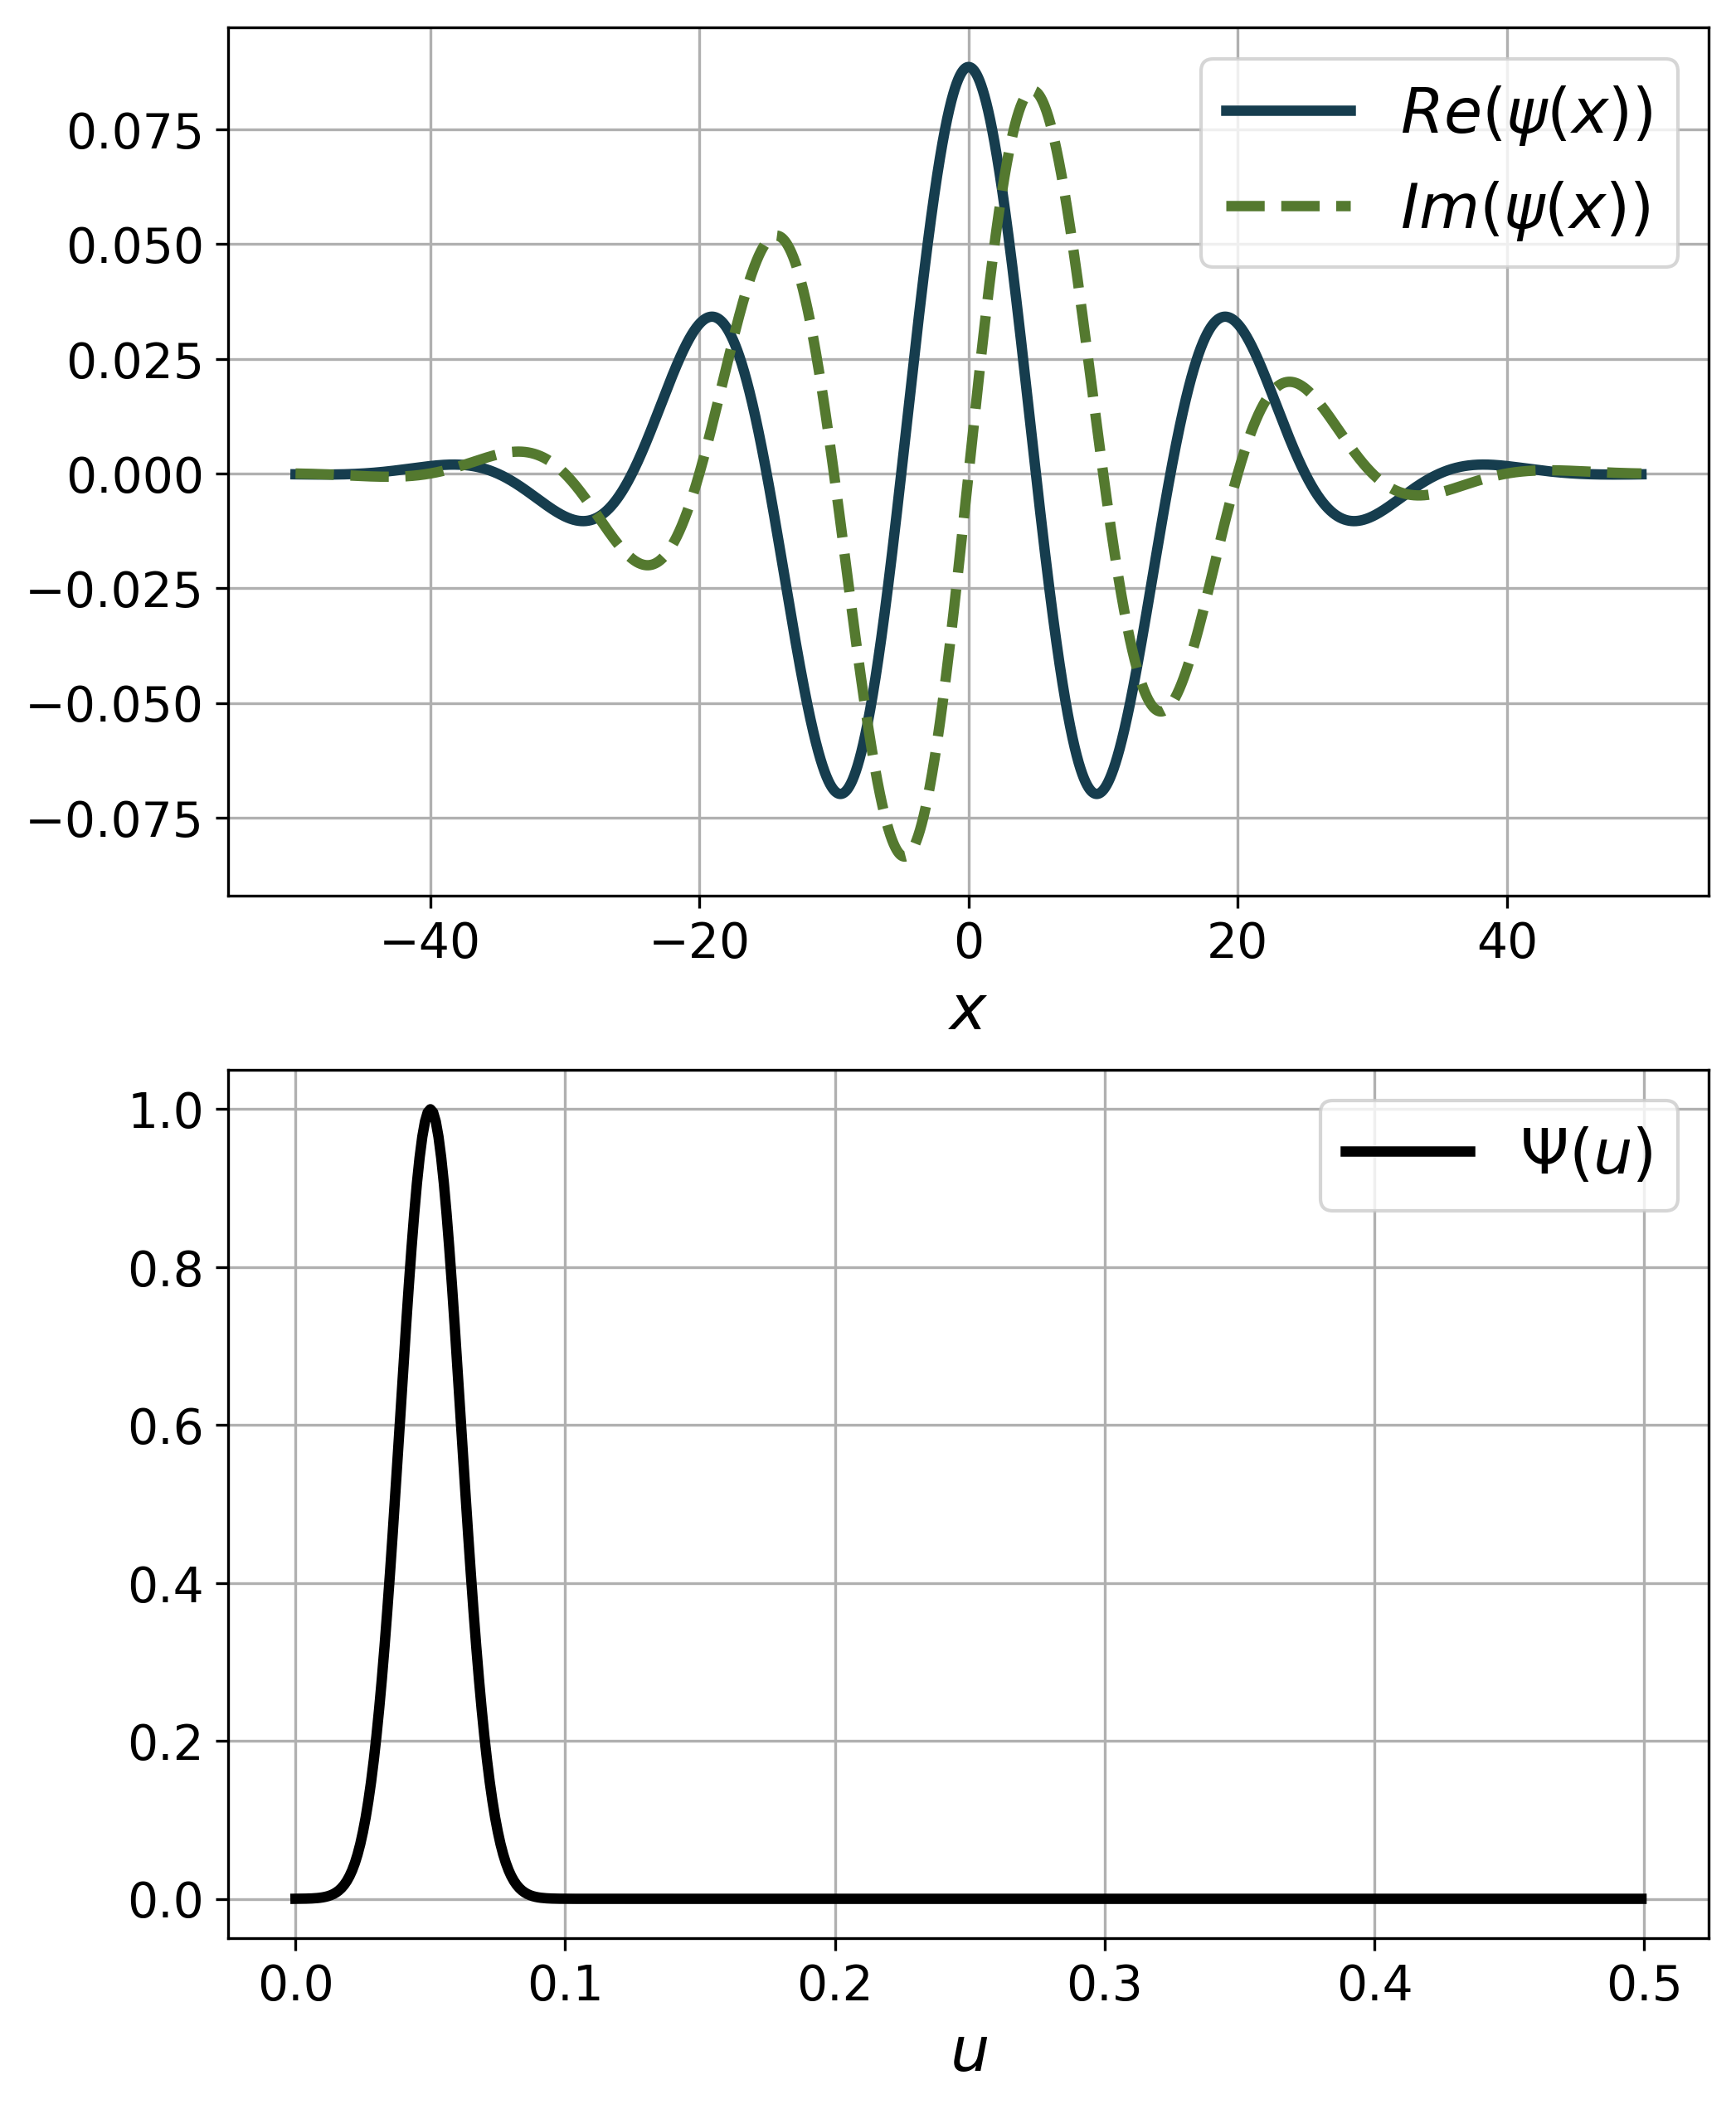
\includegraphics[width=\textwidth]{1D_GaborFilter_ver_f20_g1}
		\caption{}
		\label{fig:1D_GaborFilter_f20_g1}
	\end{subfigure}
	%add desired spacing between images, e. g. ~, \quad, \qquad, \hfill etc. 
	%(or a blank line to force the subfigure onto a new line)
	\begin{subfigure}[b]{0.23\textwidth}
		\centering
		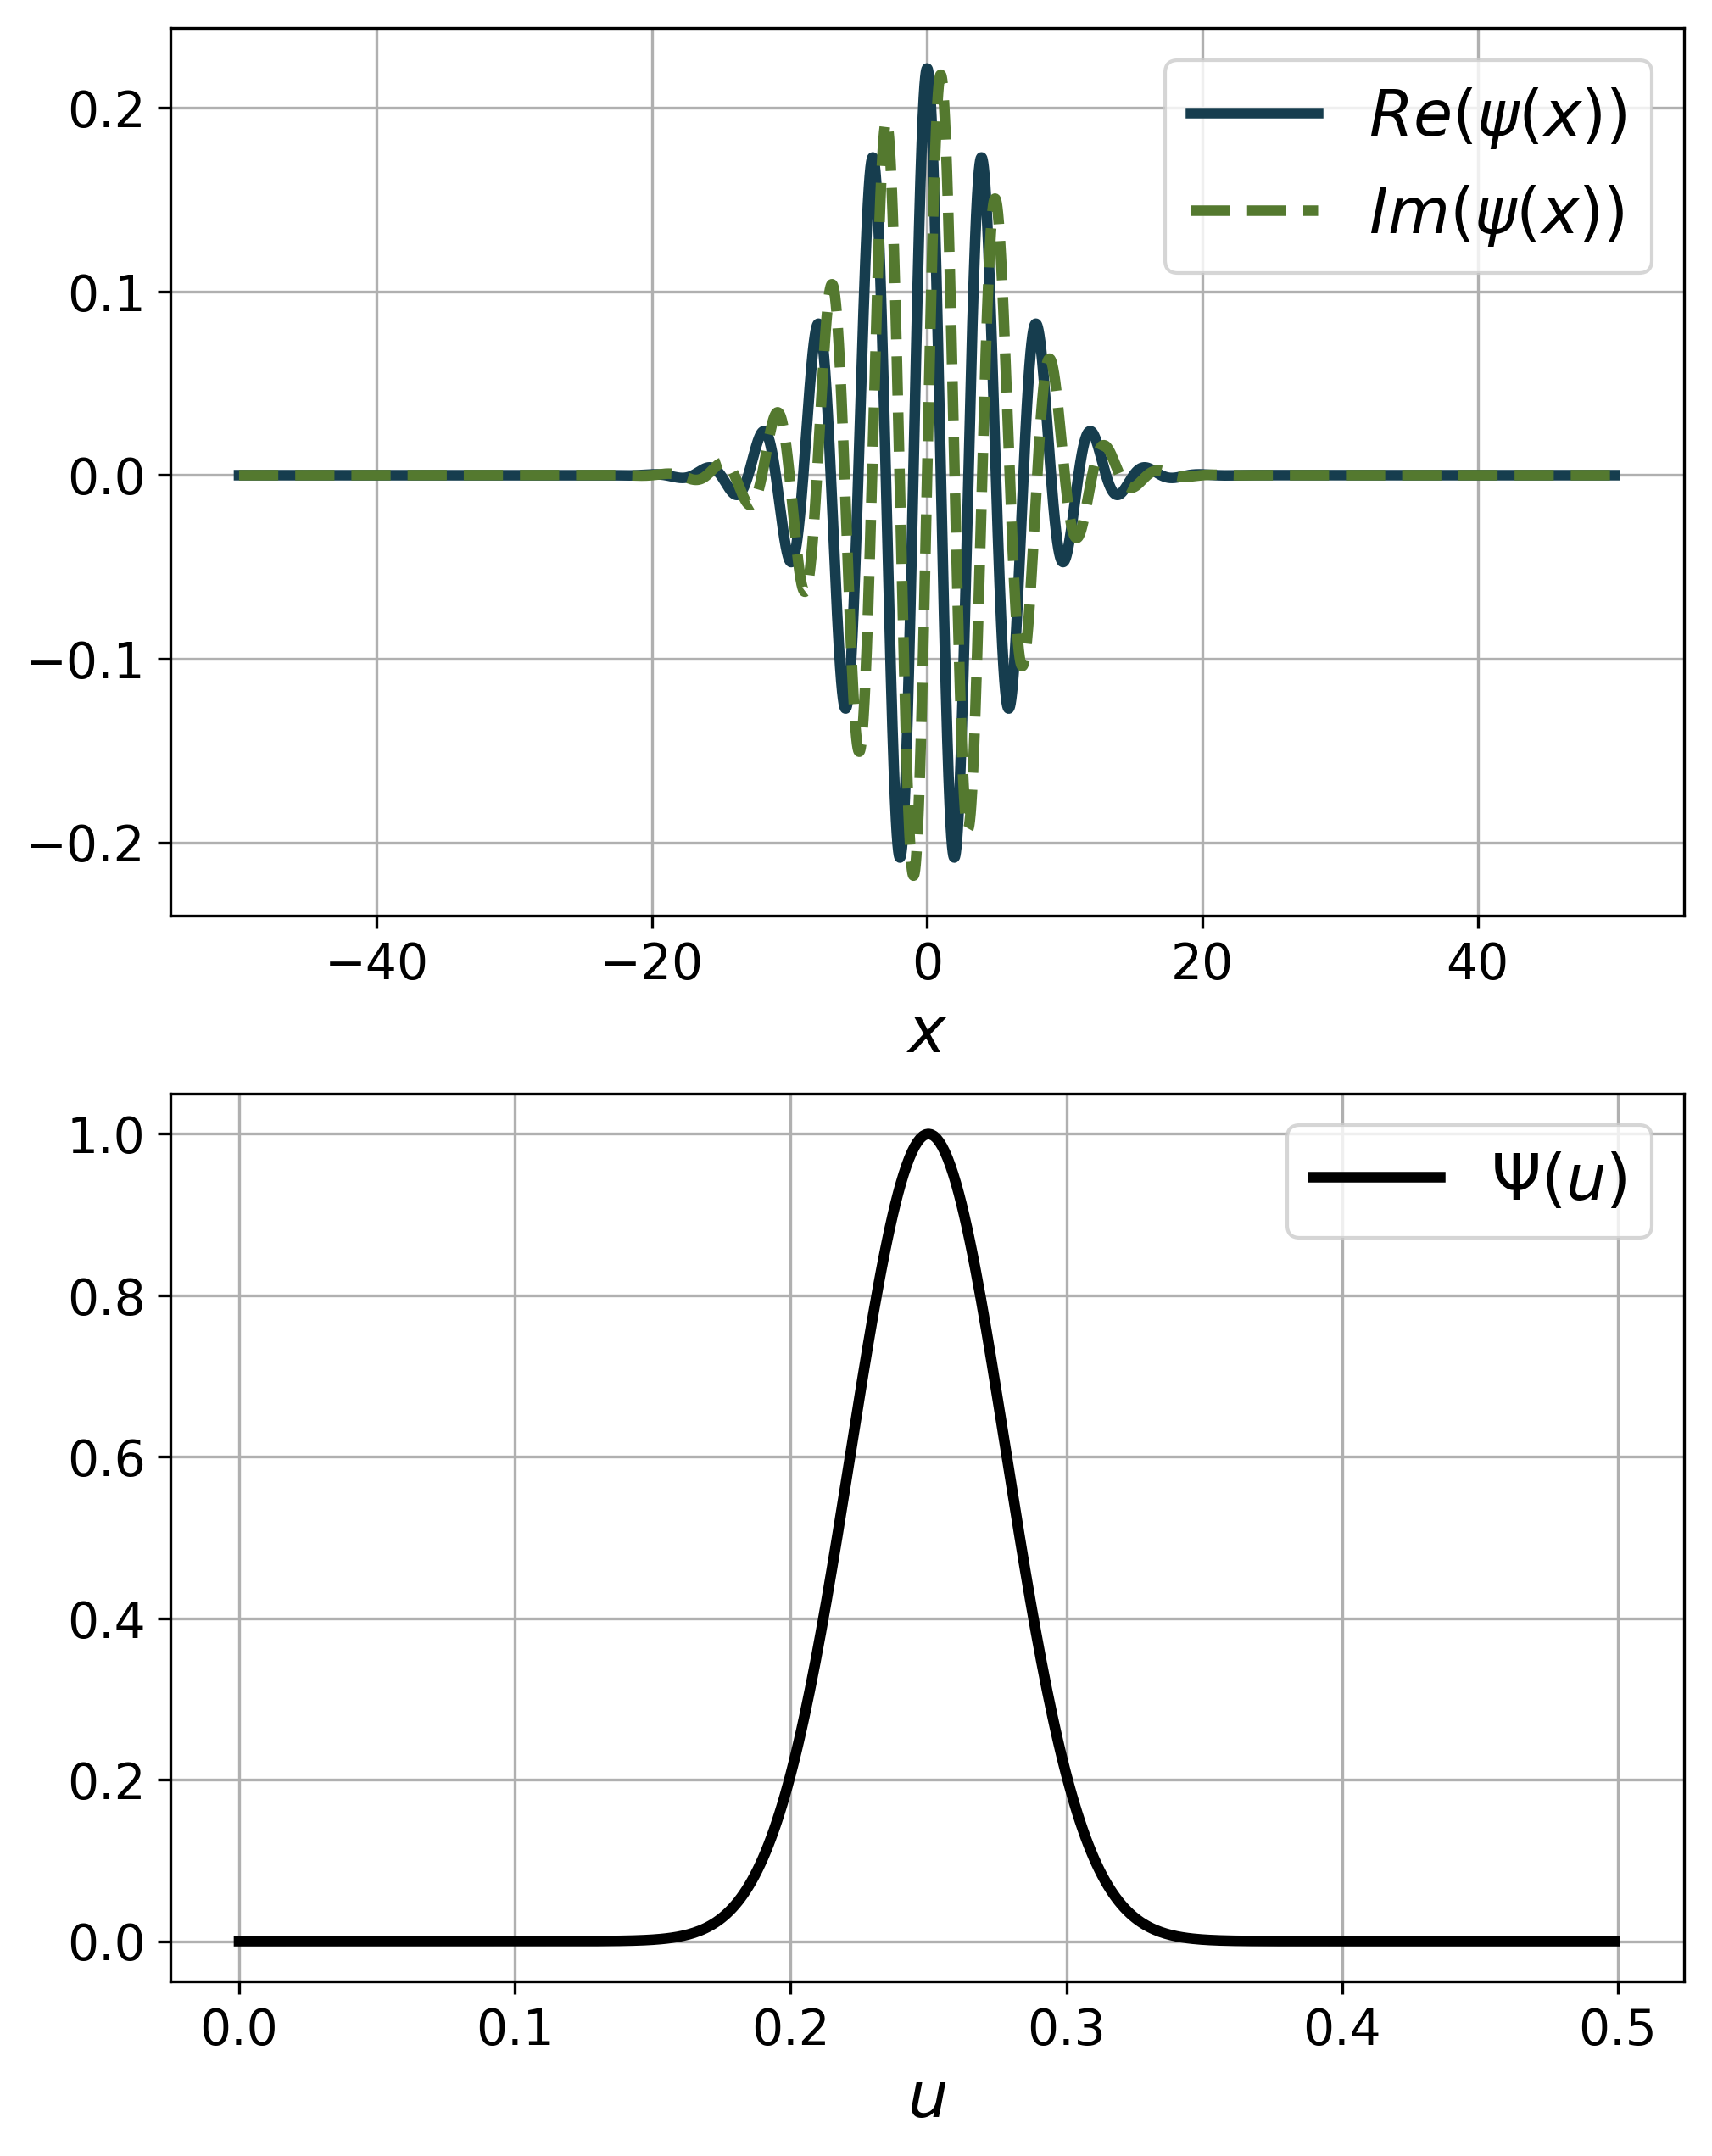
\includegraphics[width=\textwidth]{1D_GaborFilter_ver_f4_g2}
		\caption{}
		\label{fig:1D_GaborFilter_f4_g2}
	\end{subfigure}
	%add desired spacing between images, e. g. ~, \quad, \qquad, \hfill etc. 
	%(or a blank line to force the subfigure onto a new line)
	\begin{subfigure}[b]{0.23\textwidth}
		\centering
		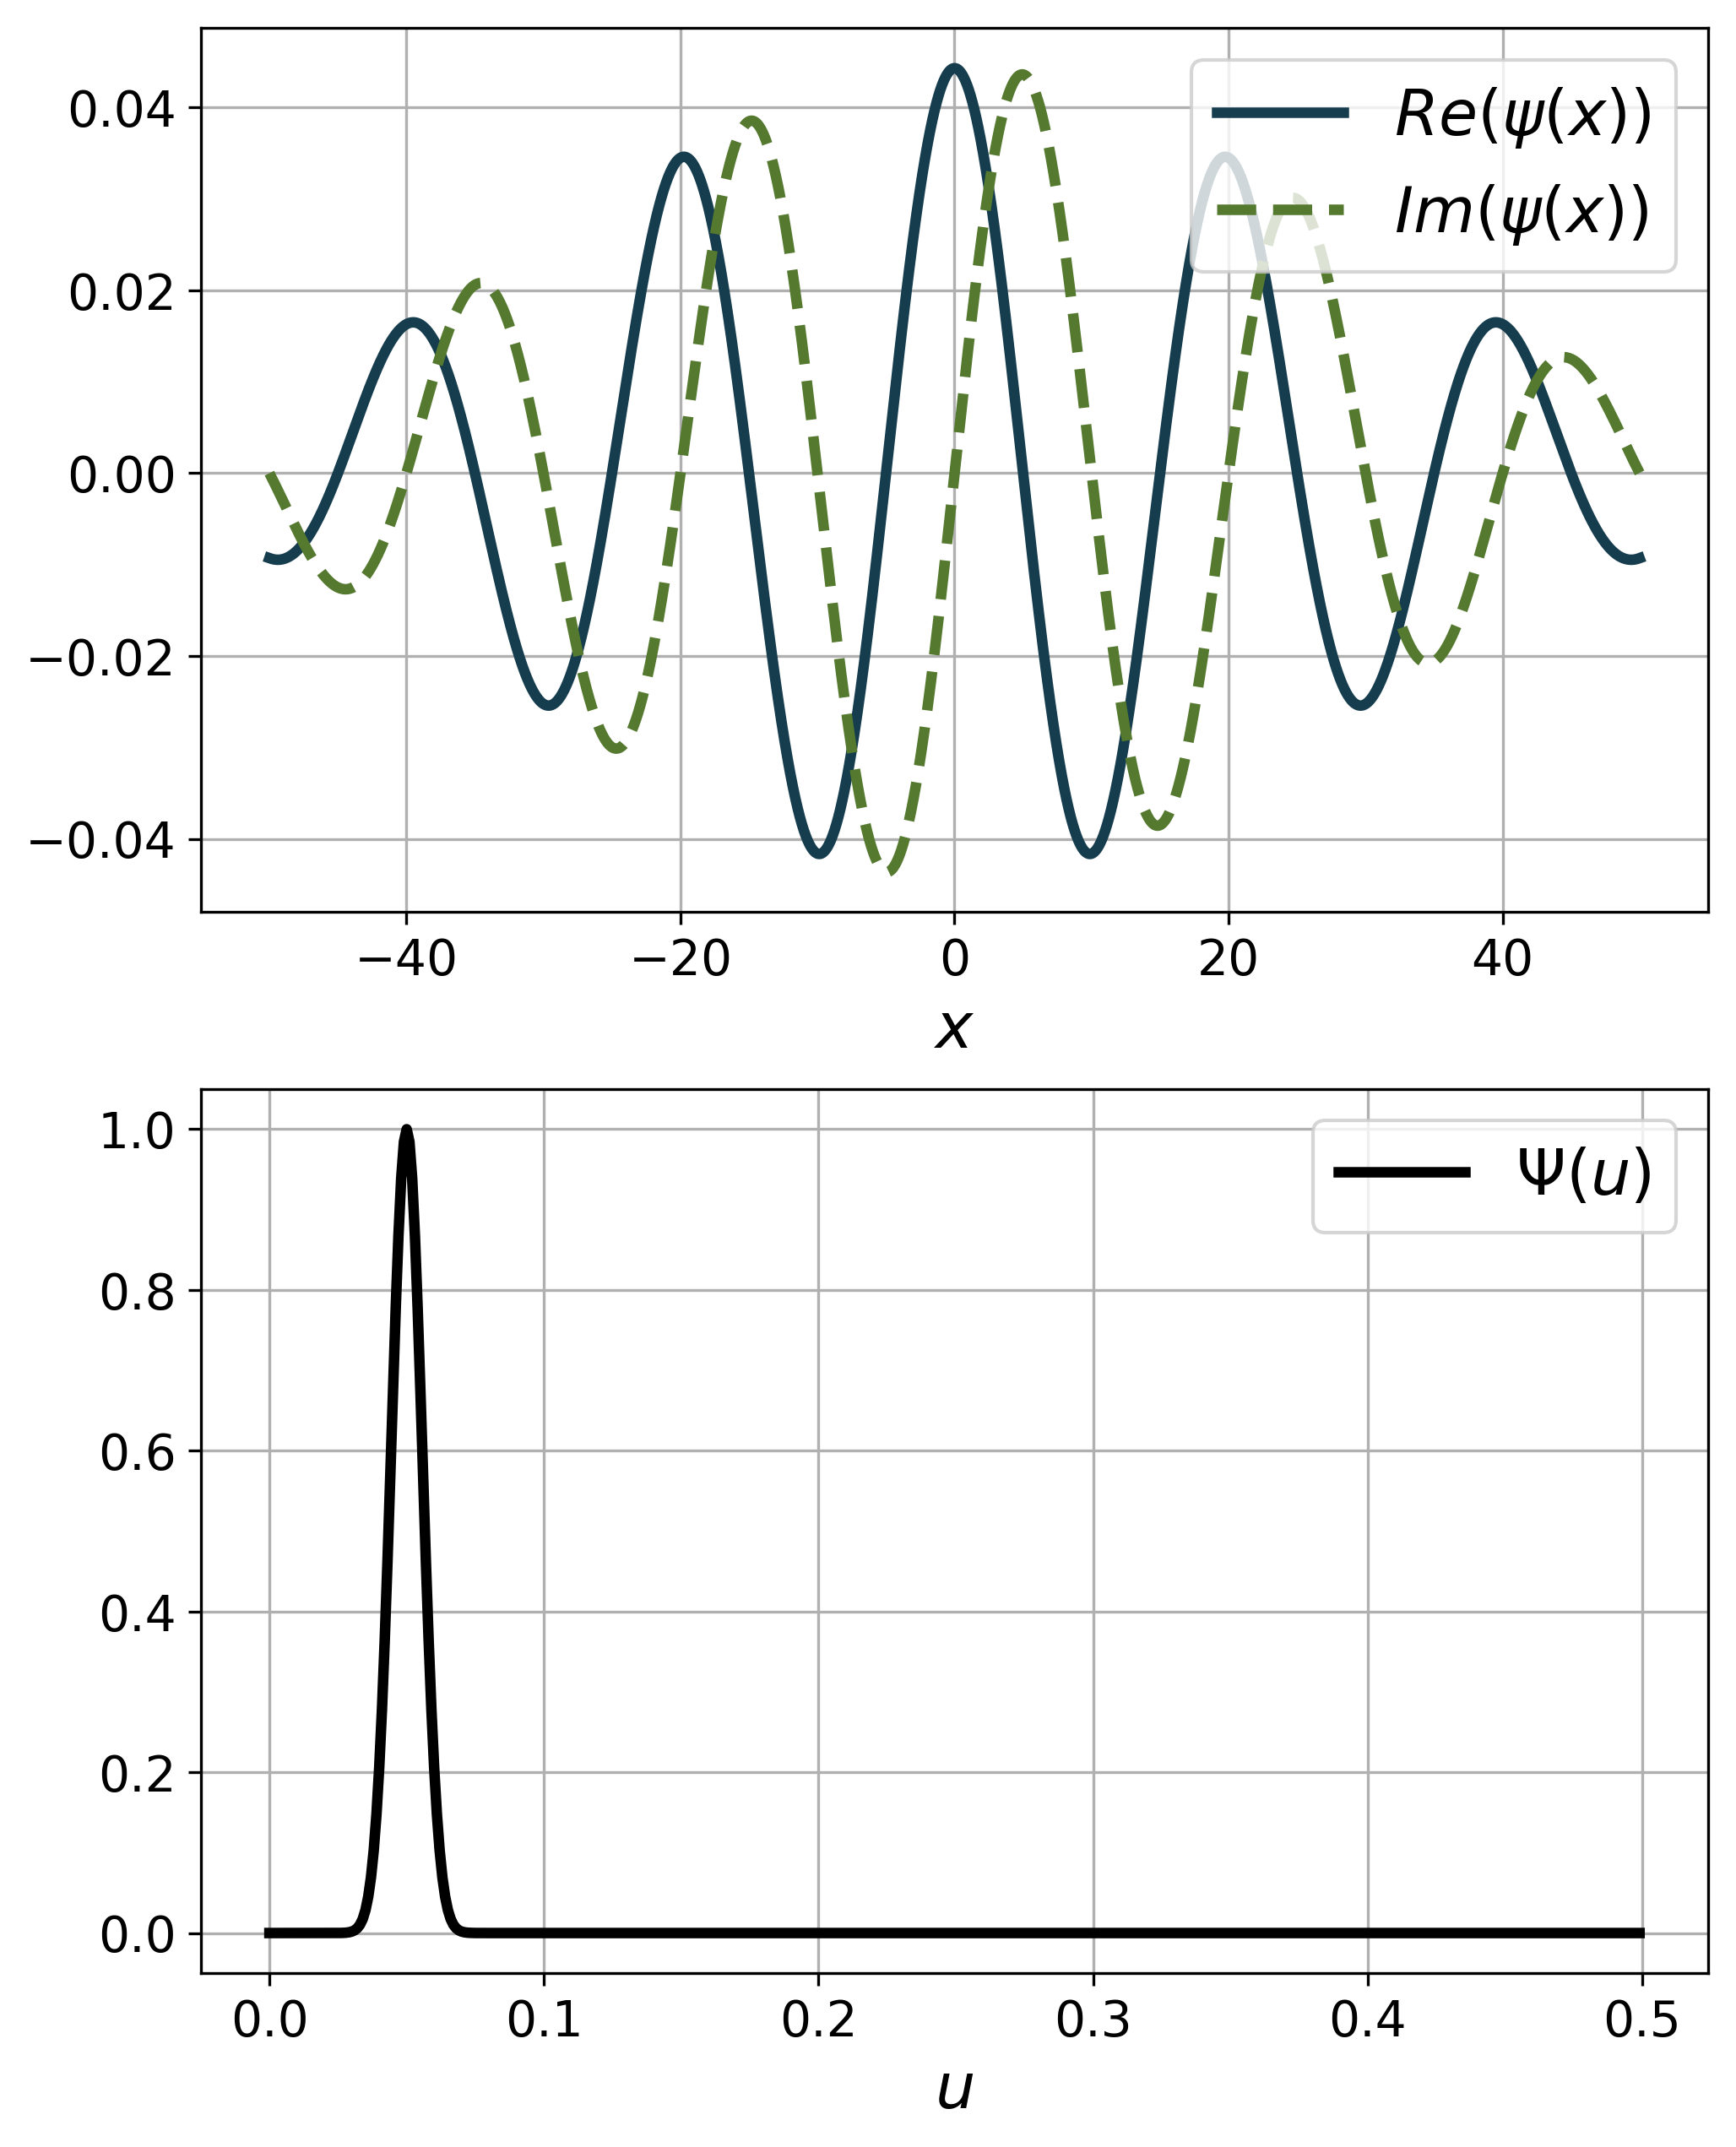
\includegraphics[width=\textwidth]{1D_GaborFilter_ver_f20_g2}
		\caption{}
		\label{fig:1D_GaborFilter_f20_g2}
	\end{subfigure}
		

  \caption{Visualization of the uncertainty principle in 1-d Gabor filters. Fist row: filters on the time domain, Second row: filters on the frequency domain. (a) $f = 1/4$, $\gamma = 1$; (b) $f = 1/20$, $\gamma = 1$; (c) $f = 1/4$, $\gamma = 2$; (d) $f = 1/20$, $\gamma = 2$.}
  \label{fig:examples_1D_GaborFilter}
\end{figure}

\subsubsection{Filter normalization} \label{subsec:filter_normalization}
The Gabor filter can be more appropriately defined by taking the following justifications. First, we must remember that we use the Gabor function as a linear filter to analyze a signal. Under this condition, the temporal analysis of the signal is carried out using the convolution operator. Considering that the Gabor function is concentrated near the time instant $t_0$ and that a convolution centered at the origin is preferable, we consider $t_0 = 0$. Since there is no evidence that any specific phase would be more beneficial than any other, another parameter that we can omit is the phase shift $\phi$. Moreover, for the functions to be similar at all locations, the phase shift should depend on the location $t_0$, and thus, the phase shift can be removed from the origin centered filter ($\phi$ = 0). Then, the Gabor filter function in its compact form is defined as 

\begin{equation}\label{eq:gabor_function_1d_timefreq_compact}
    \begin{gathered}
         g(t) =  e ^{-\alpha^2 t^2} e ^{j 2 \pi f t } \\
         G(\upsilon) =  \sqrt{\frac{\pi}{\alpha^2}} e ^{-\left(\frac{\pi}{\alpha}\right) ^{2} (\upsilon-f)^2} 
     \end{gathered}
\end{equation}

The normalization of the Gabor filter can be performed taking into account the application in which it will be used. However, in this thesis we use the general normalization which is based on the multi domain representation property of the function and following the next conditions \citep{Boukerroui.Noble.ea:JMIV:2004}:

\begin{enumerate}
    \item Maximum condition:
        \begin{equation}\label{eq:maximun_condition}
            \max{|G(\upsilon)|} = 1
        \end{equation}
    \item Constant spectra condition:
        \begin{equation}\label{eq:constant_spectrum_condition}
            \int_{-\infty}^{\infty} |g(t)| dt = 1
        \end{equation}        
\end{enumerate}

From the equation \eqref{eq:gabor_function_1d_freq}, it is evident that the maximum response of the Gabor filter in the frequency domain is a function of $\sqrt{\pi/\alpha^2}$, therefore, its inverse
\begin{equation}\label{eq:normalization_factor}
    \sqrt{\frac{\alpha^2}{\pi}}
\end{equation}
can be used as the normalization factor in the time domain and fulfill the two conditions mentioned above. Then using the normalization factor \eqref{eq:normalization_factor}, the normalized Gabor filter is defined as

\begin{equation}\label{eq:gabor_function_1d_timefreq_normalized}
    \begin{gathered}
         g(t) =  \sqrt{\frac{\alpha^2}{\pi}} e ^{-\alpha^2 t^2} e ^{j 2 \pi f t } \\
         G(\upsilon) =  e ^{-\left(\frac{\pi}{\alpha}\right) ^2 (\upsilon-f)^2}
     \end{gathered}
\end{equation}

\begin{figure}[!ht]
\centering
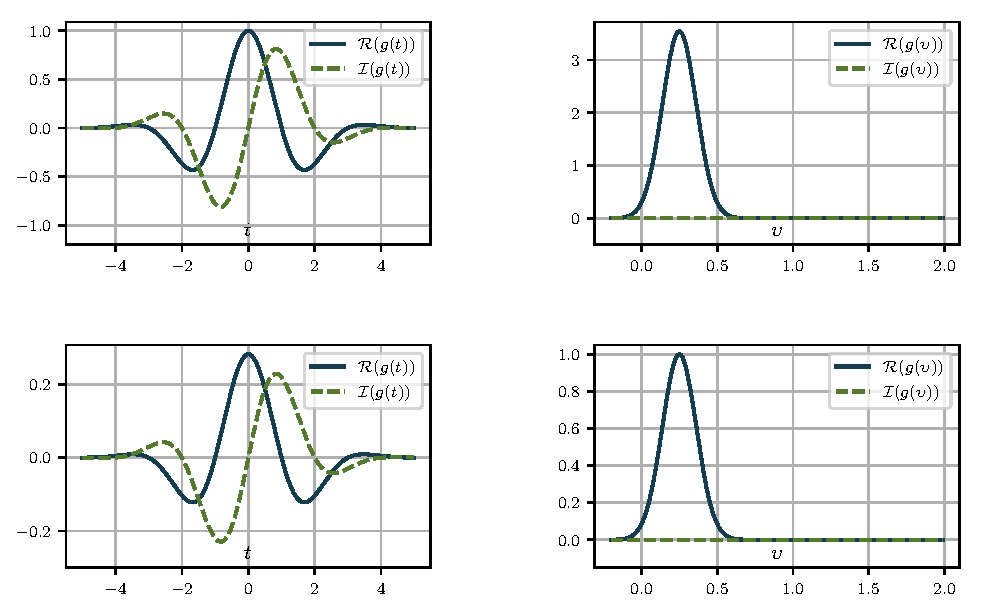
\includegraphics{GaborFilter_timefreq_1d_norm_efect.pdf}
\caption{1-d Gabor filter in the time domain (first column) and in the frequency domain (second  column). From top to bottom: non-normalized and normalized Gabor filter with [$f =1/4$, $\alpha=0.5$, $t_0=0$].}\label{fig:GaborFilter_timefreq_norm_efect}
\end{figure}

The figure \ref{fig:GaborFilter_timefreq_norm_efect} shows a Gabor filter in the time and frequency domain before and after normalization following the two conditions described above. At this point, it is important to note that normalization is an essential step in the multi-spectral analysis and the feuture extraction of a signal.

\subsubsection{Frequency filter spacing}\label{subsec:frequency_filter_spacing}
Our main interest in Gabor filters is the multispectral analysis of a function. We accomplish this by using multiple Gabor functions as filters that are tuned on several frequencies $f_m$. This group of filters is known as a Gabor filter bank. The separation between the filters bank is defined by means of the half-response spatial frequency bandwidth $B_F$ measured between two central frequencies $f_1 < f_2$ \citep{Granlund:CGIP:1978}. This bandwidth is measured in octaves and we can express it as
\begin{equation}\label{eq:octave_spacing}
    B_f = \log_2 \left( \frac{f_2}{f_1} \right)
\end{equation}

The frequency bandwidth eq. \eqref{eq:octave_spacing} shows that the central frequencies $f_m$ must have a logarithmic relationship to maintain a homogeneous spacing between the filters. The logarithmic relationship is given by a scaling factor $k=2^{B_F}$, so the frequency of each filter ($f$) in this case corresponds to the scale information. Then we can write the central frequencies as
\begin{equation}
	f_m = k^{-m} f_{max}\textrm{,} \quad m = \{1, \cdots, M\} \label{eq:filterbank_frequencies}
\end{equation} 
where $f_m$ is the $m$th frecuency, $f_{max}$ is the maximum desired frequency, $k>1$ is the frequency scaling factor and $M$ is the total number of frequencies in the filter bank.

The octave spacing between two different two adjacent filters is an interesting property of the Gabor filters, however, the filters denoted by the equations \eqref{eq:gabor_function_1d_timefreq_normalized} have a spread that only depends on the parameter $\alpha$, regardless of its central frequency $f$. This means that when implementing the Gabor function in a filter bank at different frequencies to obtain a multi-spectral decomposition of a signal, all of the filters will have the same the same spread in the frequency domain. We can see this effect in figure \ref{fig:filterbnk_octave_spacing}, where we show a filter bank with five central frequencies and an adjacent filter's spacing of one octave, that is, $M=5$ and $B_F = 1$. 


\subsubsection{Frequency crossing point}
The fact that the central frequencies $f_m$ of a filter bank are chosen to have a constant separation causes two adjacent Gabor functions to intersect at a very specific point on the frequency axis. For example, in a filter bank with two functions with central frequencies $f_1$ and $f_2$, the low cut-off frequency of the function at $f_1$ coincides with the high cut-off frequency of the function at $f_2$. Normally in the literature this crossing point $c_1$, corresponds to the points where the Gabor function has decreased half of its maximum value, i.e., $c_1= 1/2=0.5$ \citep{Granlund:CGIP:1978}. However, by setting the crossing point to half of the maximum value, the filter bank does not cover the entire spectrum of the input signal, consequently the filter bank will not respond (or the response will be minimal) to artifacts that oscillate between central frequencies. 

We obtain the mathematical expression of this crossing point $c_1$ by defining a frequency interval $\Delta f$, which represents the distance between points where the function $G(\upsilon)$ begins to decrease. A peculiarity of the Gabor function is that its analytical form in the frequency domain is completely defined by the fourier transform of the normalized Gaussian function eq. \eqref{eq:gabor_function_1d_timefreq_normalized}.

\begin{equation}\label{eq:1d_gaussian_function_freq}
    G(\upsilon) = w(\upsilon) = e ^{-\left(\frac{\pi}{\alpha}\right) ^{2} (\upsilon-f)^2}
\end{equation}
therefore, evaluating eq. \eqref{eq:1d_gaussian_function_freq} at $\upsilon = f + \frac{\Delta f}{2}$
\begin{equation}\label{eq:constant_crossing_point}
    G\left(f + \frac{\Delta f}{2}\right) = e^{-\left(\frac{\pi}{\alpha}\right)^2 \left(\frac{\Delta f}{2}\right)^2} = c_1 G(f) 
\end{equation}
we obtain the expression of the half-frequency interval 
\begin{equation}\label{eq:frequency_interval_crossing_point}
    \frac{\Delta f}{2} = \frac{\alpha}{\pi}\sqrt{\ln \left(\frac{1}{c_1}\right)}
\end{equation}
from which we obtain that the crossing point is defined as
\begin{equation}\label{eq:crossing_point}
    c_1 = e^{-\left(\frac{\alpha}{\pi} \right)^2 \left(\frac{\Delta f}{2}\right)^2 }
\end{equation}

This expression allows us to control the intersection point of two adjacent filters in the filter bank. Modifying the crossing point allows the generation of filter banks that cover (almost) the entire frequency spectrum, which translates into a more faithful decomposition of the input signal.

\subsubsection{Effective and Adaptable Gaussian Envelope}
We know that for a filter whose center frequency is $f$ and whose cut-off frequency interval is $\Delta f$, the full bandwidth expressed in octaves, $B_F$, is defined as \citep{Daugman:JOSA:1985a}.
\begin{equation}\label{eq:frequency_bandwidth_interval}
    B_F = \log_2 \left( \frac{f + \frac{\Delta f}{2} }{f - \frac{\Delta f}{2}} \right)
\end{equation}

It is clear that using the half-frequency interval eq. \eqref{eq:frequency_interval_crossing_point} into the frequency bandwidth eq. \eqref{eq:frequency_bandwidth_interval}, we find an expression that introduces a relationship between the frequency bandwidth $B_F$, the central frequency $f$ and the spread of the Gabor filter $\alpha$.
\begin{equation}\label{eq:frequency_bandwidth}
    B_F = \log_2 \left( \frac{ \frac{f}{\alpha} \pi + \sqrt{\ln \left(\frac{1}{c_1}\right)} }{ \frac{f}{\alpha} \pi - \sqrt{\ln \left(\frac{1}{c_1}\right)} } \right)
\end{equation}
The relationship is clear through the ratio 
\begin{equation}\label{eq:gamma_ratio}
    \gamma = \frac{f}{\alpha}
\end{equation}

The ratio of Eq. \ref{eq:gamma_ratio} allows to generate gabor filters of variable size as a function of the center frequency. For this, we must remember that the window size of a Gabor function is denoted by the effective width of a Gaussian function, which in the time domain has a form of
\begin{equation}\label{eq:1d_gaussian_function_time}
    w(t)=e^{-\frac{(t-t_0)^2}{2\sigma^2}}
\end{equation}

The Gaussian window Eq. \ref{eq:1d_gaussian_function_time} is infinite in extent, so it is characterized by its locality $t_0$ and its standard deviation $\sigma$, which in this context is implicit in the parameter $\alpha$ of the Gabor fuction as $\alpha^2 = 1 / 2 \sigma^2$. By setting the standard deviation dependent on the frequency ratio and the central frequency, we find that
\begin{equation}
	\sigma = \frac{\gamma}{\sqrt{2}f} \label{eq:1D_Gaussian_envelope_width}
\end{equation} 
makes Gabor's window adaptive.

In addition to adapting the filter size, with Eq. \eqref{eq:1D_Gaussian_envelope_width}, we make the Gabor filter effective, that is, we make the filter envelope correspond to the time (resp. spatial) support where the values of the function are significant. We use the empirical \textit{three-sigma} rule \cite{Pukelsheim:AMSTAT:1994}, a conventional heuristic, that expresses that nearly $99.7\%$ of the energy of the Gaussian distribution lies within three standard deviations of the mean. Therefore, we define shortest interval of the function that includes most of the energy as 
\begin{equation}
	\kappa = \lbrace p ~|~ x \in [-3\sigma, 3\sigma] \rbrace \label{eq:1D_gabor_support}
\end{equation}

The fact that the bank filters have the same width at all frequencies is not a problem nor is it a requirement to analyze a signal with the Gabor function. However, making the filter width dependent on its frequency implies a multi-resolution analysis, since the filters behave like a scaled version of each other. The advantages of and adaptative effectve envelope are related to the computation time and the loss of information when we filter a signal with a Gabor filterbank. The Fig. \ref{fig:1D_space_Gaborfilterbank} illustrates the advantages of using a filter bank with adaptive and efficient support (fig. \ref{fig:1D_space_Gaborfilterbank_env}) versus a conventional filter bank (fig. \ref{fig:1D_space_Gaborfilterbank_wo_env}). More precisely, in the case of constant envelope widht ($\kappa = \lbrace p ~|~ x \in [-50, 50] \rbrace$ for the exaple shown in fig. \ref{fig:1D_space_Gaborfilterbank_wo_env}) the computation time of responses is the same for all filter frequencies, while with the adaptive envelope, the calculation time is reduced for high frequencies since the envelope width is smaller (compare images on the first column of Fig. \ref{fig:1D_space_Gaborfilterbank}). Moreover, it exist the risk of losing information from the original signal if the chosen envelope is not large enough for low frequencies (compare images on the last column of fig. \ref{fig:1D_space_Gaborfilterbank}). Using the adaptative and effective envelope width, we recover as much energy as possible from the signal by optimizing the computation time of the response for each frequency of the filter $f_m$.

\begin{figure}[!ht] 
	\centering
	\begin{subfigure}[b]{\textwidth}
		\centering
		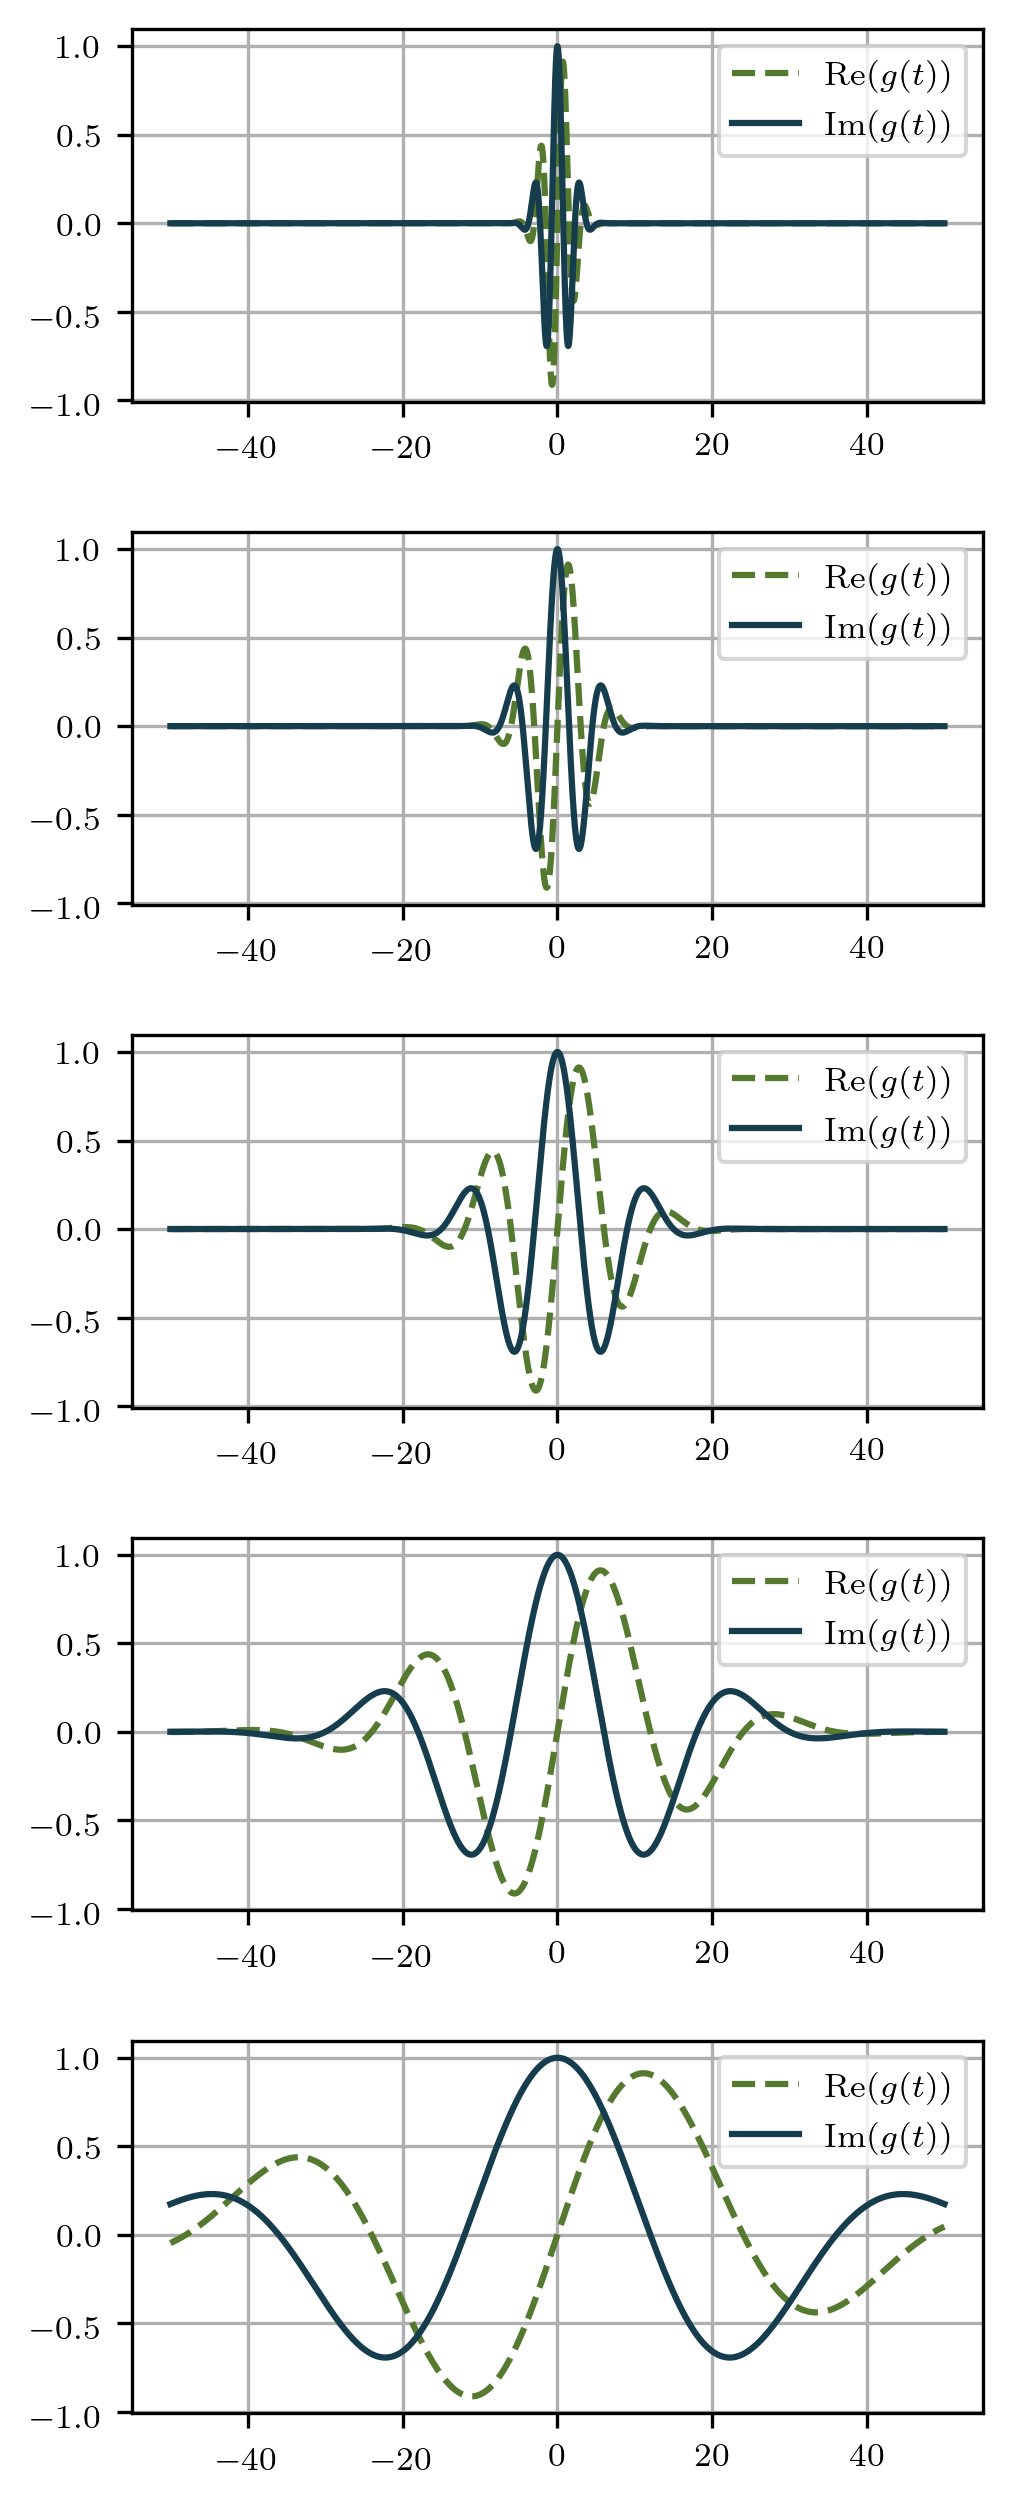
\includegraphics[width=\textwidth]{1D_space_GaborBank_m5_wo_env}
		\caption{}
		\label{fig:1D_space_Gaborfilterbank_wo_env}
	\end{subfigure}
	\qquad %add desired spacing between images, e. g. ~, \quad, \qquad, \hfill etc. 
	%(or a blank line to force the subfigure onto a new line)
	\begin{subfigure}[b]{\textwidth}
		\centering
		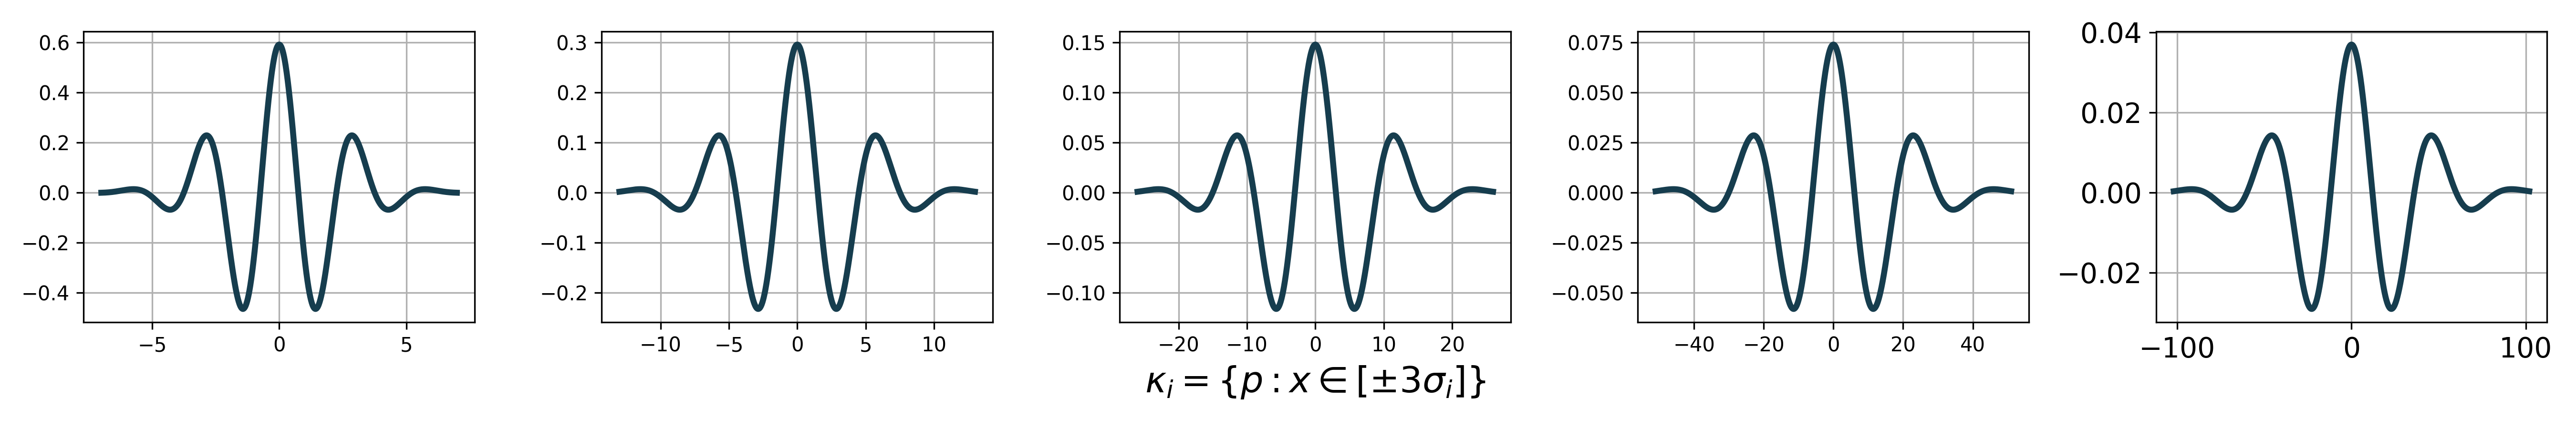
\includegraphics[width=\textwidth]{1D_space_GaborBank_m5_env}
		\caption{}
		\label{fig:1D_space_Gaborfilterbank_env}
	\end{subfigure}

  \caption{Visual representation the effective Gaussian envelope adaptation with filter bank with in  $ M = 5 $ frequencies in the space domain. (a) Filter bank with no control over the envelope, (b) Filter bank with control over the effective width of the envelope.}
  \label{fig:1D_space_Gaborfilterbank}
\end{figure}


\subsubsection{Optimized 1-d Gabor function}
Gathering the different modifications of Gabor functions enunciated in the previous sections, we can define an optimized 1-d Gabor function as follows
\begin{equation}\label{eq:gabor_function_1d_timefreq_bank}
    \begin{gathered}
         g(t) =  \frac{f}{\gamma \sqrt{\pi}} e ^{-\left(\frac{f}{\gamma}\right)^2 t^2} e ^{j 2 \pi f t } \\
         G(\upsilon) =  e ^{-\left(\frac{\gamma \pi}{f}\right) ^2 (\upsilon-f)^2}
     \end{gathered}
\end{equation}

This representation of the gabor function allows the generation of filter banks normalized by the maximum spectrum condition that are homogeneously distributed in the frequency domain. In addition, the filter bank integrates the frequency crossover point that allows quasi-total coverage of the frequency spectrum, occupying the most relevant part of the filter using an adaptive window.

The figure \ref{fig:1d_filterbank_spacing} shows shows three examples of filter banks in the frequency domain. Particulary, the figure \ref{fig:filterbnk_octave_spacing} shows a bank without the relationship between the effective width and the central frequency of the filter, whereas the figures \ref{fig:filterbnk_half_crossingpoint} and \ref{fig:filterbnk_new_crossingpoint} show the interdependence between $\alpha$, $B_F$, $f$ and $c_1$ and the behavior of the bank with a different crossing point.

\begin{figure}[!ht]
\centering
    \subcaptionbox{\label{fig:filterbnk_octave_spacing}}{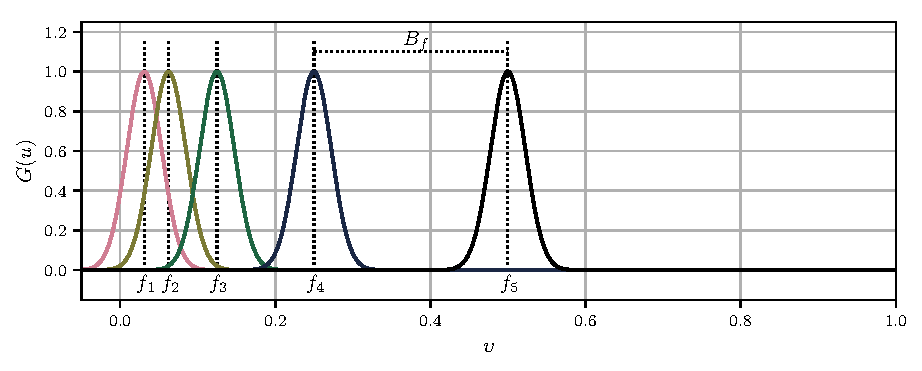
\includegraphics[width=\textwidth]{GaborFilterbank_freq_1d_octave_spacing.pdf}} \\
    \subcaptionbox{\label{fig:filterbnk_half_crossingpoint}}{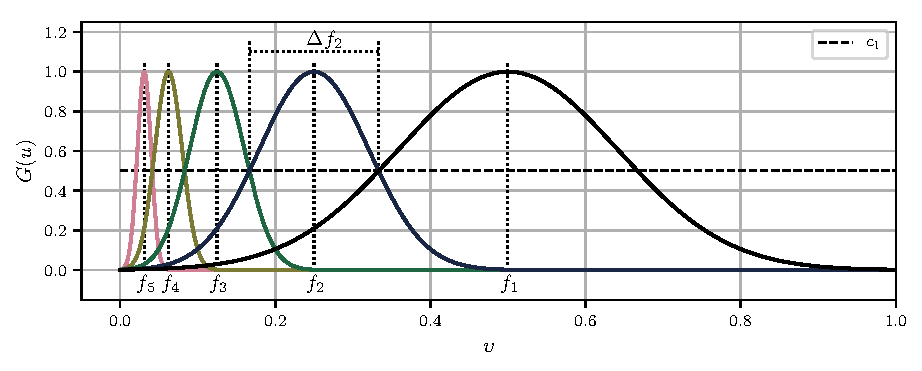
\includegraphics[width=\textwidth]{GaborFilterbank_freq_1d_half_crossingpoint.pdf}}\\
    \subcaptionbox{\label{fig:filterbnk_new_crossingpoint}}{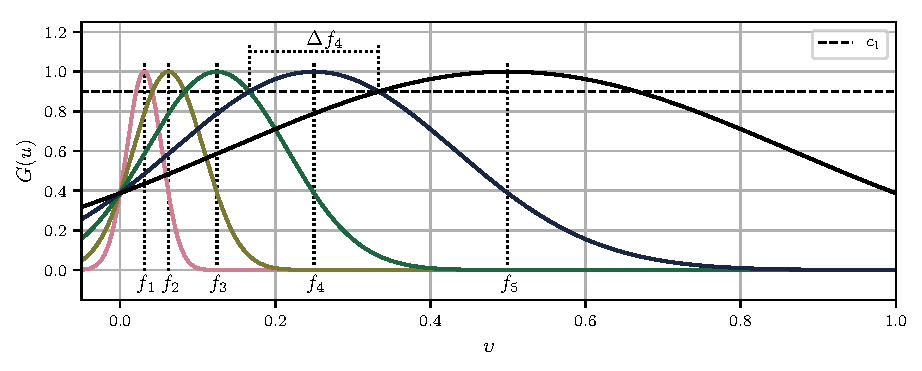
\includegraphics[width=\textwidth]{GaborFilterbank_freq_1d_new_crossingpoint.pdf}}
\caption{Filter spacing and crossing point effect represented on a bank of filters in the frequency domain: (a) Separation of filters in octaves without crossing point between adjacent filters $[B_F=1, \alpha=0.1, c_1=-]$, (b) High and low cut-off frequency points given by $\Delta f$ $[B_F=1, \alpha=f/\gamma, c_1=0.5]$, (c) Filter bank behavior after changing the crossing point $[B_F=1, \alpha=f/\gamma, c_1=0.9]$.}\label{fig:1d_filterbank_spacing}
\end{figure}


\subsection{2-d Gabor filters}
The generalization of the Gabor function's theory from 1-d to 2-d is straightforward. First, we replace the time variable $t$ with the pair of spatial coordinates $(x, y)$ and the frequency variable $f$ with the pair of frequency variables $(u, v)$. Then, as for the 1-d case, the 2-d Gabor functions follows the Heinsenberg principle where the uncertainty measures for the space and spatial-frequency domains are expressed in terms of $\Delta x$, $\Delta y$, $\Delta u$, and $\Delta v$, for which it holds that

\begin{equation}\label{eq:uncertainty_principle_2d}
    \begin{gathered}
        \Delta x\Delta u \geq \frac{1}{4\pi}\textrm{,} \quad \Delta y\Delta v \geq \frac{1}{4\pi}\textrm{and} \quad \Delta x \Delta y \Delta u \Delta v \geq \frac{1}{16\pi^2}
    \end{gathered}
\end{equation}

In the 2-d case, the Gabor function is represented by the modulated product of a harmonic oscillation on any spatial frequency and any orientation, represented by a complex exponential, with a pulse in the form of a probability function, represented by an elliptical Gaussian ellipse on any orientation. For simplicity, it can be assumed that the orientation of the Gaussian and the harmonic modulation are the same and  therefore, define a compact form of the 2-d GEF in the space domain applying the given simplifications as follows
\begin{equation}\label{eq:gabor_function_2d_space_compact}
    \begin{gathered}
        g(x, r) =  e ^{-\left(\alpha^2 x_r^2 + \beta^2 y_r^2\right)} e ^{j 2 \pi f x_r } \\
        x_r = x \cos{\theta} + y \sin{\theta}\\
        y_r = -x \sin{\theta} + y \cos{\theta}
     \end{gathered}
\end{equation}
whereas the analytical expression for the 2-d GEF in the spatial-frequency domain is obtained from the Fourier transform of \eqref{eq:gabor_function_2d_space_compact}, $G(u, v) = \mathcal{F}\{g(x, y)\}$, and is given by 
\begin{equation}\label{eq:gabor_function_2d_frequency_compact}
    \begin{gathered}
        G(u, v) =  \frac{\pi}{\alpha \beta} e ^{- \pi^2 \left(\frac{\left( u_r - f\right)^2}{\alpha^2} + \frac{v_r^2}{\beta^2}\right)} \\
        u_r = u \cos{\theta} + v \sin{\theta}\\
        v_r = -u \sin{\theta} + v \cos{\theta}
     \end{gathered}
\end{equation}

The two above expressions can be normalized by following the same reasoning as in the 1-d case. We apply the maximum value condition \eqref{eq:maximun_condition} and the constant spectrum condition \eqref{eq:constant_spectrum_condition} described in Section \ref{subsec:filter_normalization} to get $\max{|G(u,v)|} = 1$ and $\int_{-\infty}^{\infty} \int_{-\infty}^{\infty} |g(x,y)| dx dy = 1$ for a filter on any frequency $f$ and orientation $\theta$. 
Under these circumstances, the normalization constant is defined by
\begin{equation}\label{eq:normalization_constant_2d}
    \frac{\alpha \beta}{\pi}
\end{equation}
which applied to equations \eqref{eq:gabor_function_2d_space_compact}  and \eqref{eq:gabor_function_2d_frequency_compact}, gives us the normalized Gabor function in both 2-d domains. 

\begin{equation}\label{eq:gabor_function_2d_spacefrequency_normalized}
    \begin{gathered}
        g(x, r) = \frac{\alpha \beta}{\pi} e ^{-\left(\alpha^2 x_r^2 + \beta^2 y_r^2\right)} e ^{j 2 \pi f x_r } \\
        G(u, v) =   e ^{- \pi^2 \left(\frac{\left( u_r - f\right)^2}{\alpha^2} + \frac{v_r^2}{\beta^2}\right)} 
     \end{gathered}
\end{equation}

\subsubsection{Orientation filter spacing}

Equivalently than its 1-d version, the Gabor functions defined by equations \eqref{eq:gabor_function_2d_spacefrequency_normalized} does not cover most of the spectrum when they are used to generate a filter bank at different frequencies and orientations (see Figure \ref{fig:2d_filterbank_octave_spacing}). Therefore it is not useful for the reconstruction of a signal and/or the extraction of features. To obtain a more encompassing filter bank, it is evident that we need to include a relationship between the sharpness of the Gaussian window and the central frequency. 

The sharpness of the Gaussian function, unlike the 1-d case, now includes two variables ($\alpha, \beta$) that affect the effective width of the Gabor filter envelope. Such an envelope can have an elliptical shape, where $\alpha $ controls the length of the major axis and $\beta$ controls the length of the minor axis. 

The analysis of the frequency separation between adjacent filters of a bank viewed in the Section \ref{subsec:frequency_filter_spacing} is also valid in the 2-d case. Thus, the full bandwidth of half the frequency response, $B_F$, represents the separation between the center frequencies; the interval $\Delta f$ represents the distance between the points where $G(u, v)$ begins to decrease and; the full frequency bandwidth through the ratio $\gamma$ and the crossing point $c_1$ allows adapting the size of the major axis of the envelope $\alpha$ depending on the center frequency $f$.

We can do a similar analysis for the minor axis of Gabor's envelope. First, notice that insertion of the orientation variable $\theta$ in the 2-d case implies the existence of an angular separation $B_{\Theta}$ between the centers of the filters in a bank (see Figure \ref{fig:2d_filterbank_octave_spacing}). This angular bandwidth can be defined by the total number of orientations $N$ in a filter bank such that
\begin{equation}\label{eq:angular_bandwidth}
    B_{\theta} = \frac{\pi}{N}
\end{equation}

We propose to vary the length of $\beta$ as a function of the central frequency and the angular bandwidth through an angular interval $\Delta \theta$, which is the distance along $\beta$ where $G(u, v)$ begins to decrease.

\begin{equation}\label{eq:orientation_interval_crossing_point}
    \frac{\Delta \theta}{2} = \frac{\beta}{\pi}\sqrt{\ln \left(\frac{1}{c_2}\right)}
\end{equation}

We know that for a filter whose center frequency is $f$ and whose cut-off angular interval is $\Delta \theta$, the full orientation bandwidth $B_\Theta$ expressed in radians is defined as \citep{Daugman:JOSA:1985a}.
\begin{equation}\label{eq:orientation_bandwidth_interval}
    B_{\theta} = 2 \tan^{-1} \left( \frac{\Delta \theta}{2f} \right)
\end{equation}

It is clear that using expression \eqref{eq:orientation_interval_crossing_point} in equation \eqref{eq:orientation_bandwidth_interval}, we find the expression that relates the frequency bandwidth to the central frequency and the length of the Gaussian minor axis.
\begin{equation}\label{eq:orientation_bandwidth}
    B_{\theta} = 2 \tan^{-1} \left( \frac{\beta}{\pi f} \sqrt{\ln \left(\frac{1}{c_2}\right)} \right)
\end{equation}

Taking the above relationships permits to write the 2-d GEF to use it into a bank as follows. 

\begin{equation}\label{eq:gabor_function_2d_spacefreq_bank}
    \begin{gathered}
         g(x,y) =  \frac{f^2}{\gamma \eta \pi} e ^{-\left(\frac{f^2}{\gamma^2} x_r^2 + \frac{f^2}{\eta^2} y_r^2\right)} e ^{j 2 \pi f x_r } \\
         G(u,v) =  e ^{-\left(\frac{\pi}{f}\right)^2\left( \gamma^2 (u_r-f)^2 + \eta^2 v_r^2\right)}
     \end{gathered}
\end{equation}
where now the length $\alpha$ of each filter in the bank will be determined based on the ratio $\gamma = \frac{f}{\alpha}$ and crossing point between adjacent filters $c_1$; and the length $\beta$ will be determined based on the ratio $\eta = \frac{f}{\beta}$ and crossing point between adjacent filters $c_2$.

The figure \ref{fig:2d_filterbank_spacing} shows the octave spacing and the orientation bandwidth for a bank of filters in the frequency domain. Particulary, the figure \ref{fig:2d_filterbank_octave_spacing} shows a bank without the relationship between the effective width and the central frequency of the filter, whereas the figures \ref{fig:filterbank_half_crossingpoint} show the interdependence between $\alpha$, $\beta$, $B_F$, $B_{\theta}$, $f$ and the crossing points $c_1$, $c_2$.

\begin{figure}[!ht]
\centering
    \subcaptionbox{\label{fig:2d_filterbank_octave_spacing}}{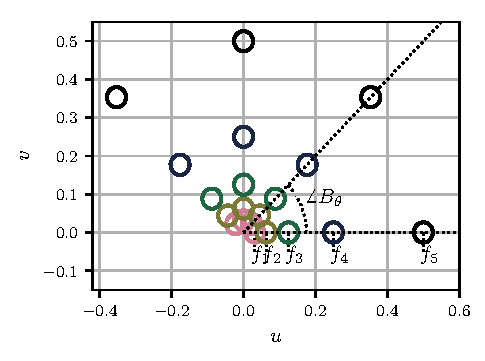
\includegraphics[width=0.49\textwidth]{GaborFilterbank_freq_2d_octave_spacing.pdf}}
    \subcaptionbox{\label{fig:2d_filterbank_half_crossingpoint}}{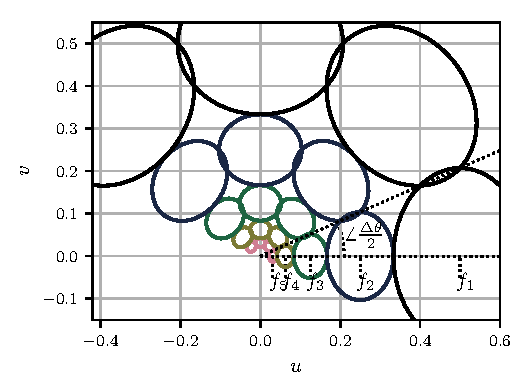
\includegraphics[width=0.49\textwidth]{GaborFilterbank_freq_2d_half_crossingpoint.pdf}}    
\caption{Filter spacing and crossing point effect represented on a bank of filters in the frequency domain: (a) Separation of 2-d filters without crossing points between adjacent filters $[B_F=1, B_{\theta} = 45^{\circ}, \alpha=\beta=0.1, c_1=c_2=-]$, (b) High and low cut-off frequency points given by $\Delta f$ and $\Delta \theta$ $[B_F=1, B_{\theta} = 45^{\circ}, \alpha=f/\gamma, \beta=f/\eta, c_1=c_2=0.5]$.}\label{fig:2d_filterbank_spacing}
\end{figure}

\section{Conclusion}

\begin{figure}[!ht]
\centering
    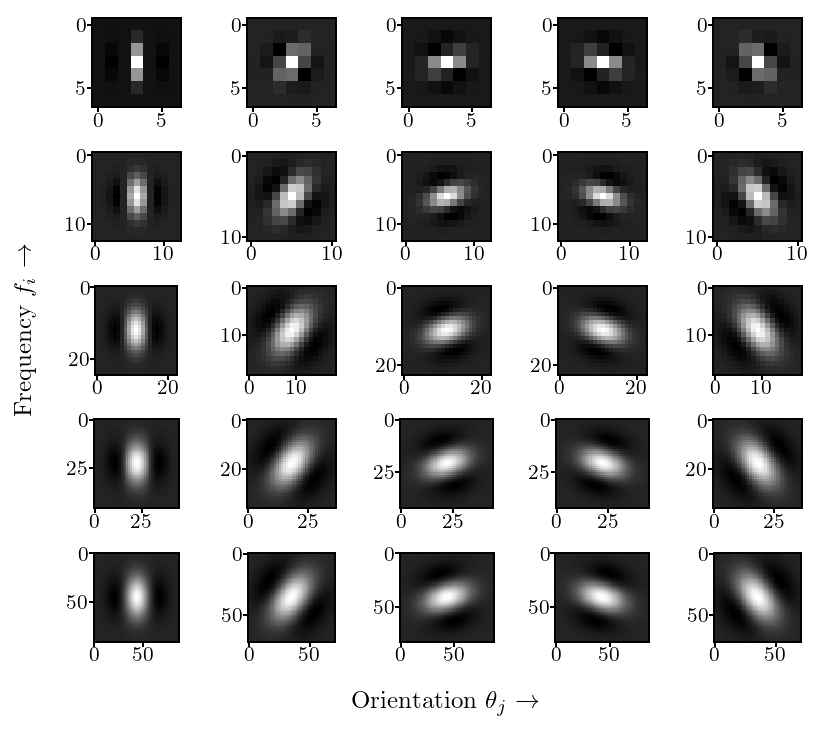
\includegraphics[width=\textwidth]{GaborFilterbank_spatial_2d}
    \caption{Real part of a custom designed Gabor filter bank. The design parameters are: max/min period $[1/f_{min}=70, 1/f_{max}=4]$, crossing points (frequency and angular) $[c_1=c_2=-0.9]$, bandwidths (frequency and angular) $[B_F=1, B_{\theta} = 35^{\circ}]$, standard devaitions $[\sigma=3]$.}\label{fig:2d_filterbank}
\end{figure}